
% Figure weak selection
\begin{figure}
\hspace{-2cm}\begin{tabular}{ccc}
\subfigure[Death-Birth \label{fig:EXDB}]{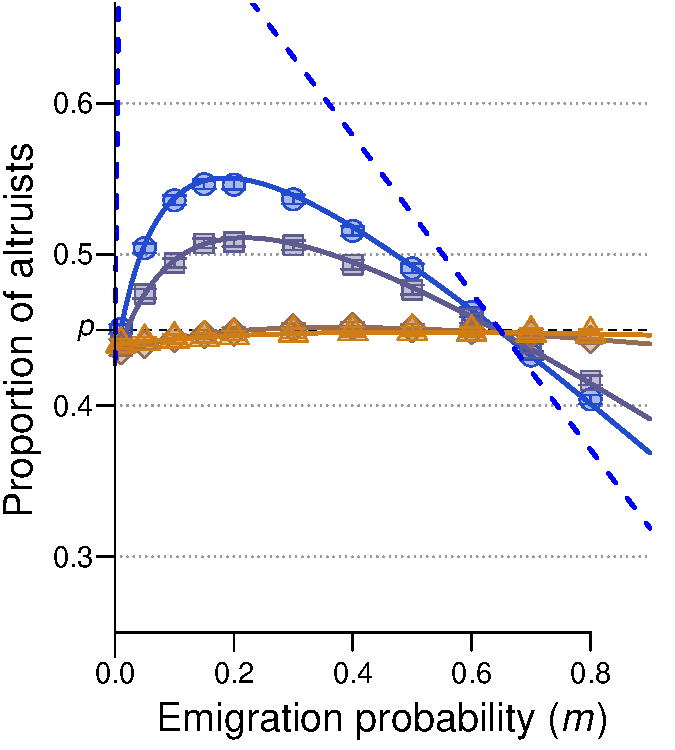
\includegraphics[type=pdf,ext=.pdf,read=.pdf, width=\wpic]{../Programs/R/Pics/EXDB_sel0.005_htg0}}
&
\subfigure[Birth-Death \label{fig:EXBD}]{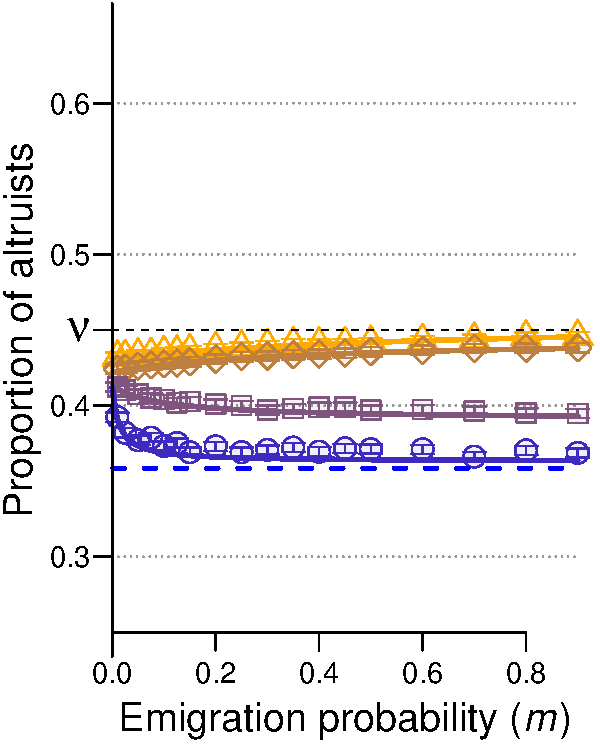
\includegraphics[type=pdf,ext=.pdf,read=.pdf, width=\wpic]{../Programs/R/Pics/EXBD_sel0.005_htg0}}
&
\subfigure[Wright-Fisher \label{fig:EXWF}]{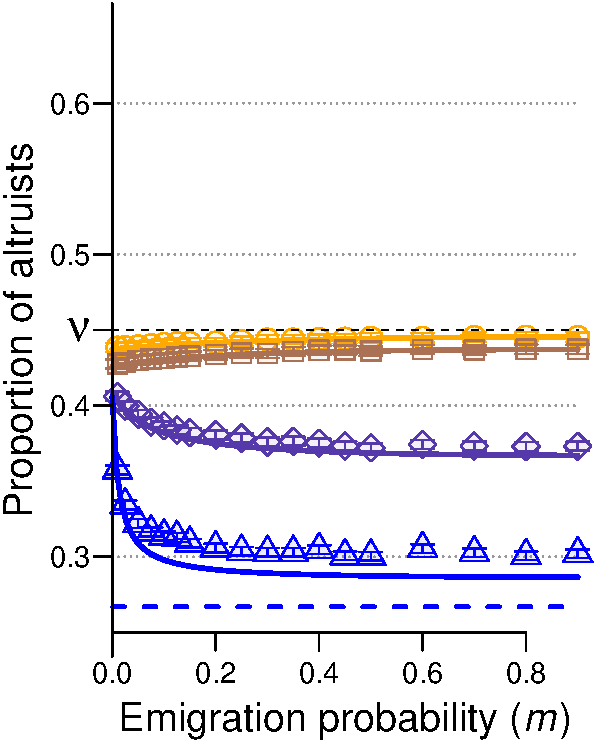
\includegraphics[type=pdf,ext=.pdf,read=.pdf, width=\wpic]{../Programs/R/Pics/EXWF_sel0.005_htg0}}
\end{tabular}
\caption{Expected proportion of altruists under weak selection, as a function of the emigration probability $m$, for different mutation values ($\mu = 0.001$ (blue, dots), $0.01$ (purple, squares), $0.1$ (brown, diamonds), $0.25$ (orange, triangles); the dashed blue lines correspond to $\mu=0$) and different life-cycles (\subref{fig:EXDB} Moran Death-Birth, \subref{fig:EXBD} Moran Birth Death, \subref{fig:EXWF} Wright-Fisher). The curves are the analytical results, the points are the output of numerical simulations. 
Parameters: $\selstr = 0.005$, $\mutbias=0.45$, $b = 15$, $c = 1$, $n=4$ individuals per deme, $\ndemes=15$ demes.}
\label{fig:EX}
\end{figure}